\hypertarget{mrtimers_8h}{
\section{mrtimers.h File Reference}
\label{mrtimers_8h}\index{mrtimers.h@{mrtimers.h}}
}


This graph shows which files directly or indirectly include this file:\begin{figure}[H]
\begin{center}
\leavevmode
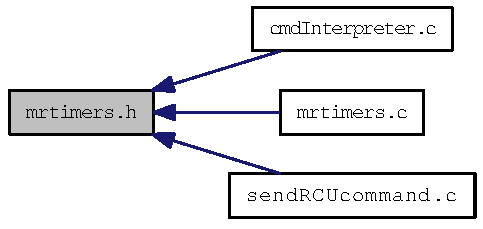
\includegraphics[width=134pt]{mrtimers_8h__dep__incl}
\end{center}
\end{figure}
\subsection*{Typedefs}
\begin{CompactItemize}
\item 
typedef void($\ast$) \hyperlink{mrtimers_8h_9c199b5712594663db80db9a9ec6d6e0}{mr\-Timer\-Handler\_\-t} (int)
\end{CompactItemize}
\subsection*{Functions}
\begin{CompactItemize}
\item 
int \hyperlink{mrtimers_8h_bf67f427f962506bad53c7ade379249c}{init\-MRTimers} (int i\-Base\-Time)
\item 
int \hyperlink{mrtimers_8h_7ce639af18d4674cf8e9ad36b95e76da}{release\-MRTimers} ()
\item 
int \hyperlink{mrtimers_8h_42192584a948fab8215173b75a4991b7}{set\-MRTimer\-Debug\-Flag} (int i\-Flag)
\item 
int \hyperlink{mrtimers_8h_53329aecf5a990cc91ae4355794f32ed}{clear\-MRTimer\-Debug\-Flag} (int i\-Flag)
\item 
int \hyperlink{mrtimers_8h_ccfd598b6f1a3ca5599e8bc3588d1cf7}{start\-Timer} (int i\-Type)
\item 
int \hyperlink{mrtimers_8h_bca69eeff549afdd7d72c0d011eea863}{set\-Timer\-Handler} (int id, int i\-Time\-Out\-Sec, int i\-Time\-Out\-Usec, \hyperlink{mrtimers_8h_9c199b5712594663db80db9a9ec6d6e0}{mr\-Timer\-Handler\_\-t} handler)
\item 
int \hyperlink{mrtimers_8h_fa991349587b8e300e5363a21dcee3b7}{stop\-Timer} (int id)
\item 
int \hyperlink{mrtimers_8h_60a100d9612c31984637866c7e975958}{get\-Timer\-Value} (int id, int $\ast$p\-Sec, int $\ast$p\-Usec)
\item 
const char $\ast$ \hyperlink{mrtimers_8h_eec88b57f56b75bdef646c5e44e0c2dc}{get\-Timer\-Value\-String} (int id)
\end{CompactItemize}


\subsection{Typedef Documentation}
\hypertarget{mrtimers_8h_9c199b5712594663db80db9a9ec6d6e0}{
\index{mrtimers.h@{mrtimers.h}!mrTimerHandler_t@{mrTimerHandler\_\-t}}
\index{mrTimerHandler_t@{mrTimerHandler\_\-t}!mrtimers.h@{mrtimers.h}}
\subsubsection[mrTimerHandler\_\-t]{\setlength{\rightskip}{0pt plus 5cm}typedef void($\ast$) \hyperlink{mrtimers_8h_9c199b5712594663db80db9a9ec6d6e0}{mr\-Timer\-Handler\_\-t}(int)}}
\label{mrtimers_8h_9c199b5712594663db80db9a9ec6d6e0}




Definition at line 22 of file mrtimers.h.

\subsection{Function Documentation}
\hypertarget{mrtimers_8h_53329aecf5a990cc91ae4355794f32ed}{
\index{mrtimers.h@{mrtimers.h}!clearMRTimerDebugFlag@{clearMRTimerDebugFlag}}
\index{clearMRTimerDebugFlag@{clearMRTimerDebugFlag}!mrtimers.h@{mrtimers.h}}
\subsubsection[clearMRTimerDebugFlag]{\setlength{\rightskip}{0pt plus 5cm}int clear\-MRTimer\-Debug\-Flag (int {\em i\-Flag})}}
\label{mrtimers_8h_53329aecf5a990cc91ae4355794f32ed}




Definition at line 254 of file mrtimers.c.

References g\_\-MRTdbg\-Flags.

Referenced by execute\-Main\-Commands().\hypertarget{mrtimers_8h_60a100d9612c31984637866c7e975958}{
\index{mrtimers.h@{mrtimers.h}!getTimerValue@{getTimerValue}}
\index{getTimerValue@{getTimerValue}!mrtimers.h@{mrtimers.h}}
\subsubsection[getTimerValue]{\setlength{\rightskip}{0pt plus 5cm}int get\-Timer\-Value (int {\em id}, int $\ast$ {\em p\-Sec}, int $\ast$ {\em p\-Usec})}}
\label{mrtimers_8h_60a100d9612c31984637866c7e975958}




Definition at line 285 of file mrtimers.c.

References TMRSys\-Timer::cycle\-Count, find\-Timer\-Entry(), g\_\-MRTdbg\-Flags, g\_\-systimers, MRT\_\-DBG\_\-TIMER\_\-MSG, TMRTimer::startcycle, TMRTimer::startvalue, and TMRTimer::type\-Index.

Referenced by get\-Timer\-Value\-String(), timed\-Wait(), and wait\-Condition().

Here is the call graph for this function:\begin{figure}[H]
\begin{center}
\leavevmode
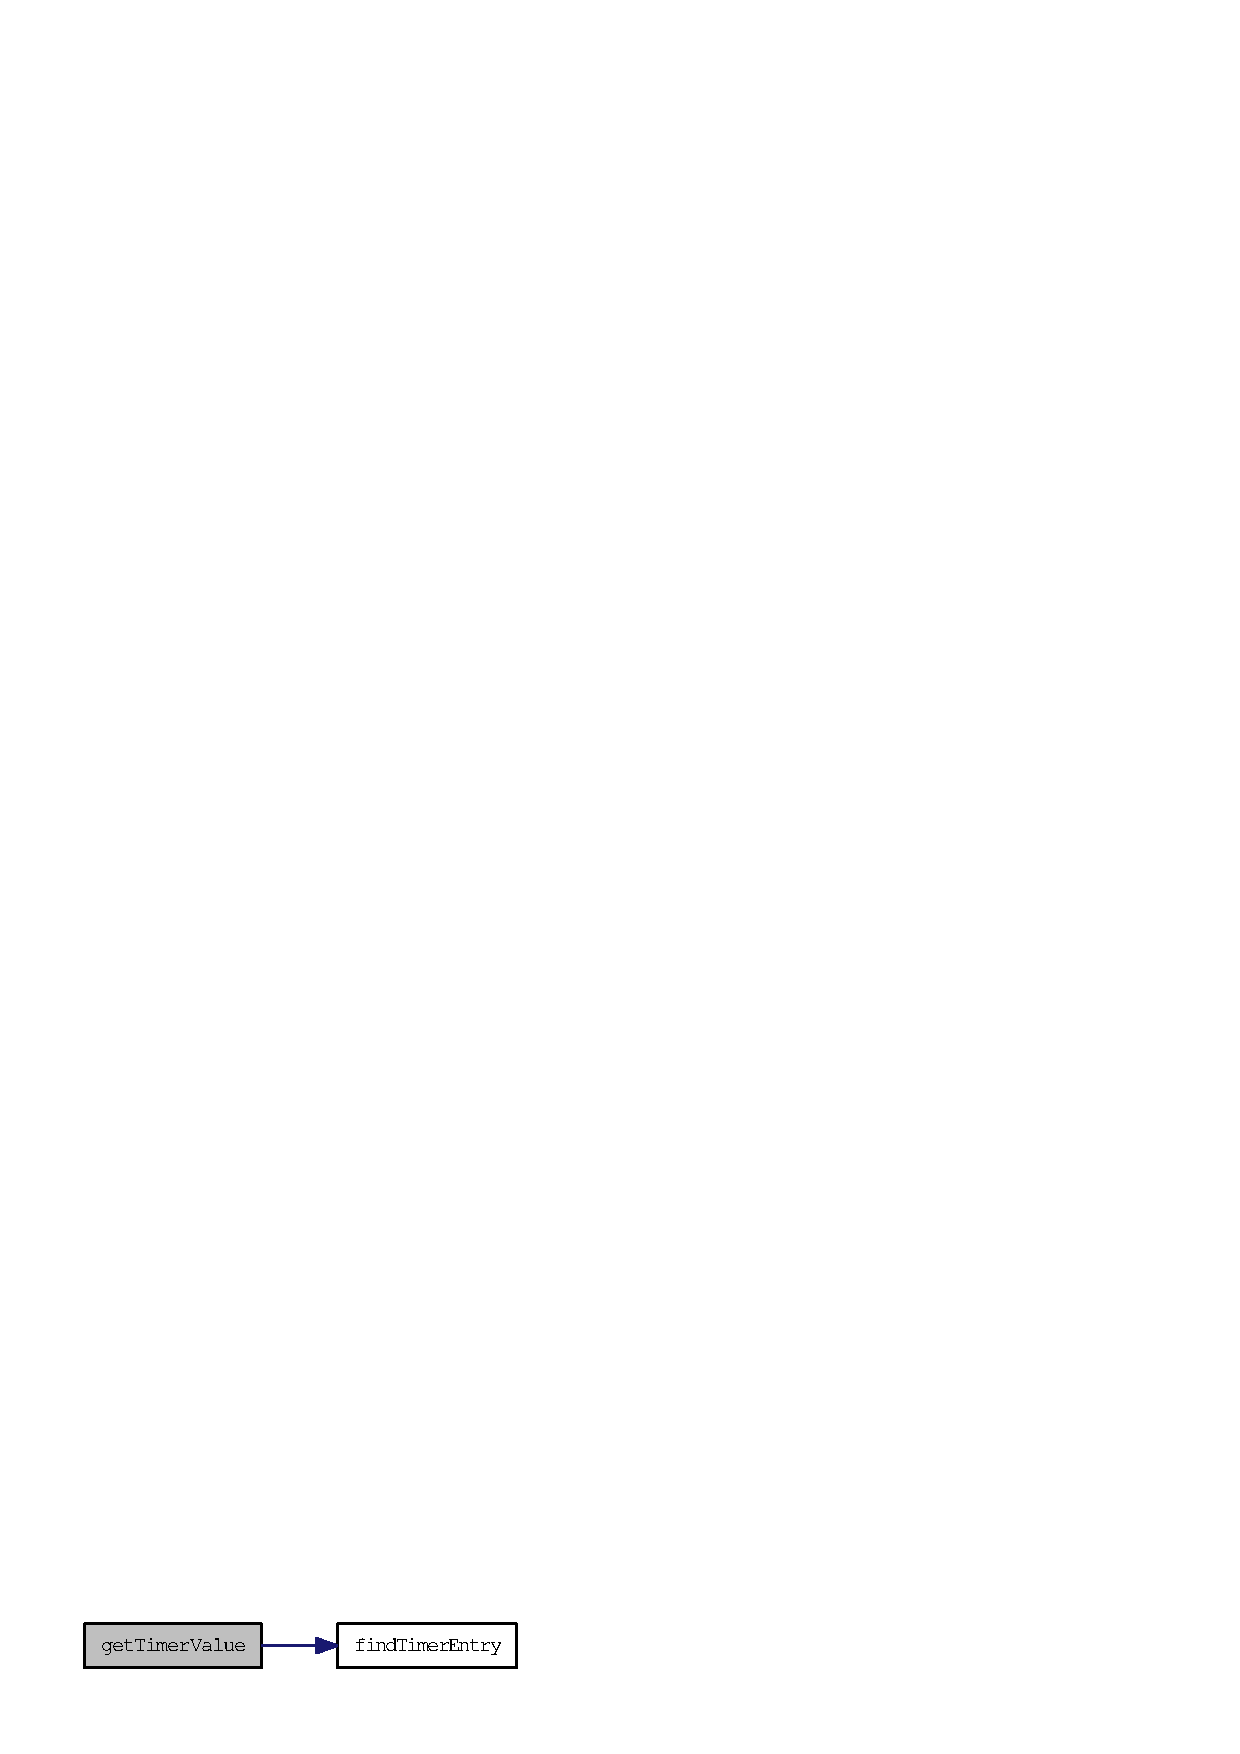
\includegraphics[width=126pt]{mrtimers_8h_60a100d9612c31984637866c7e975958_cgraph}
\end{center}
\end{figure}
\hypertarget{mrtimers_8h_eec88b57f56b75bdef646c5e44e0c2dc}{
\index{mrtimers.h@{mrtimers.h}!getTimerValueString@{getTimerValueString}}
\index{getTimerValueString@{getTimerValueString}!mrtimers.h@{mrtimers.h}}
\subsubsection[getTimerValueString]{\setlength{\rightskip}{0pt plus 5cm}const char$\ast$ get\-Timer\-Value\-String (int {\em id})}}
\label{mrtimers_8h_eec88b57f56b75bdef646c5e44e0c2dc}




Definition at line 323 of file mrtimers.c.

References g\_\-str\-Time, and get\-Timer\-Value().

Referenced by exec\-Batch(), and exec\-Write\-Cmd().

Here is the call graph for this function:\begin{figure}[H]
\begin{center}
\leavevmode
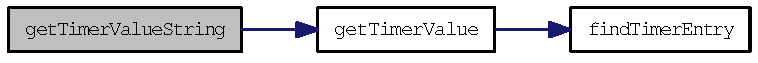
\includegraphics[width=200pt]{mrtimers_8h_eec88b57f56b75bdef646c5e44e0c2dc_cgraph}
\end{center}
\end{figure}
\hypertarget{mrtimers_8h_bf67f427f962506bad53c7ade379249c}{
\index{mrtimers.h@{mrtimers.h}!initMRTimers@{initMRTimers}}
\index{initMRTimers@{initMRTimers}!mrtimers.h@{mrtimers.h}}
\subsubsection[initMRTimers]{\setlength{\rightskip}{0pt plus 5cm}int init\-MRTimers (int {\em i\-Base\-Time})}}
\label{mrtimers_8h_bf67f427f962506bad53c7ade379249c}




Definition at line 184 of file mrtimers.c.

References TMRSys\-Timer::cycle\-Count, g\_\-array\-Timers, g\_\-array\-Timer\-Size, g\_\-MRTdbg\-Flags, g\_\-signal\-Handler, g\_\-signals, g\_\-systimers, g\_\-systimertypes, and MRT\_\-DBG\_\-INIT\_\-MSG.

Referenced by main().\hypertarget{mrtimers_8h_7ce639af18d4674cf8e9ad36b95e76da}{
\index{mrtimers.h@{mrtimers.h}!releaseMRTimers@{releaseMRTimers}}
\index{releaseMRTimers@{releaseMRTimers}!mrtimers.h@{mrtimers.h}}
\subsubsection[releaseMRTimers]{\setlength{\rightskip}{0pt plus 5cm}int release\-MRTimers ()}}
\label{mrtimers_8h_7ce639af18d4674cf8e9ad36b95e76da}




Definition at line 236 of file mrtimers.c.

References g\_\-array\-Timers, and g\_\-array\-Timer\-Size.

Referenced by main().\hypertarget{mrtimers_8h_42192584a948fab8215173b75a4991b7}{
\index{mrtimers.h@{mrtimers.h}!setMRTimerDebugFlag@{setMRTimerDebugFlag}}
\index{setMRTimerDebugFlag@{setMRTimerDebugFlag}!mrtimers.h@{mrtimers.h}}
\subsubsection[setMRTimerDebugFlag]{\setlength{\rightskip}{0pt plus 5cm}int set\-MRTimer\-Debug\-Flag (int {\em i\-Flag})}}
\label{mrtimers_8h_42192584a948fab8215173b75a4991b7}




Definition at line 248 of file mrtimers.c.

References g\_\-MRTdbg\-Flags.

Referenced by execute\-Main\-Commands().\hypertarget{mrtimers_8h_bca69eeff549afdd7d72c0d011eea863}{
\index{mrtimers.h@{mrtimers.h}!setTimerHandler@{setTimerHandler}}
\index{setTimerHandler@{setTimerHandler}!mrtimers.h@{mrtimers.h}}
\subsubsection[setTimerHandler]{\setlength{\rightskip}{0pt plus 5cm}int set\-Timer\-Handler (int {\em id}, int {\em i\-Time\-Out\-Sec}, int {\em i\-Time\-Out\-Usec}, \hyperlink{mrtimers_8h_9c199b5712594663db80db9a9ec6d6e0}{mr\-Timer\-Handler\_\-t} {\em handler})}}
\label{mrtimers_8h_bca69eeff549afdd7d72c0d011eea863}




Definition at line 273 of file mrtimers.c.\hypertarget{mrtimers_8h_ccfd598b6f1a3ca5599e8bc3588d1cf7}{
\index{mrtimers.h@{mrtimers.h}!startTimer@{startTimer}}
\index{startTimer@{startTimer}!mrtimers.h@{mrtimers.h}}
\subsubsection[startTimer]{\setlength{\rightskip}{0pt plus 5cm}int start\-Timer (int {\em i\-Type})}}
\label{mrtimers_8h_ccfd598b6f1a3ca5599e8bc3588d1cf7}




Definition at line 260 of file mrtimers.c.

References create\-Timer(), and find\-Timer\-Entry().

Referenced by exec\-Batch(), exec\-Write\-Cmd(), timed\-Wait(), and wait\-Condition().

Here is the call graph for this function:\begin{figure}[H]
\begin{center}
\leavevmode
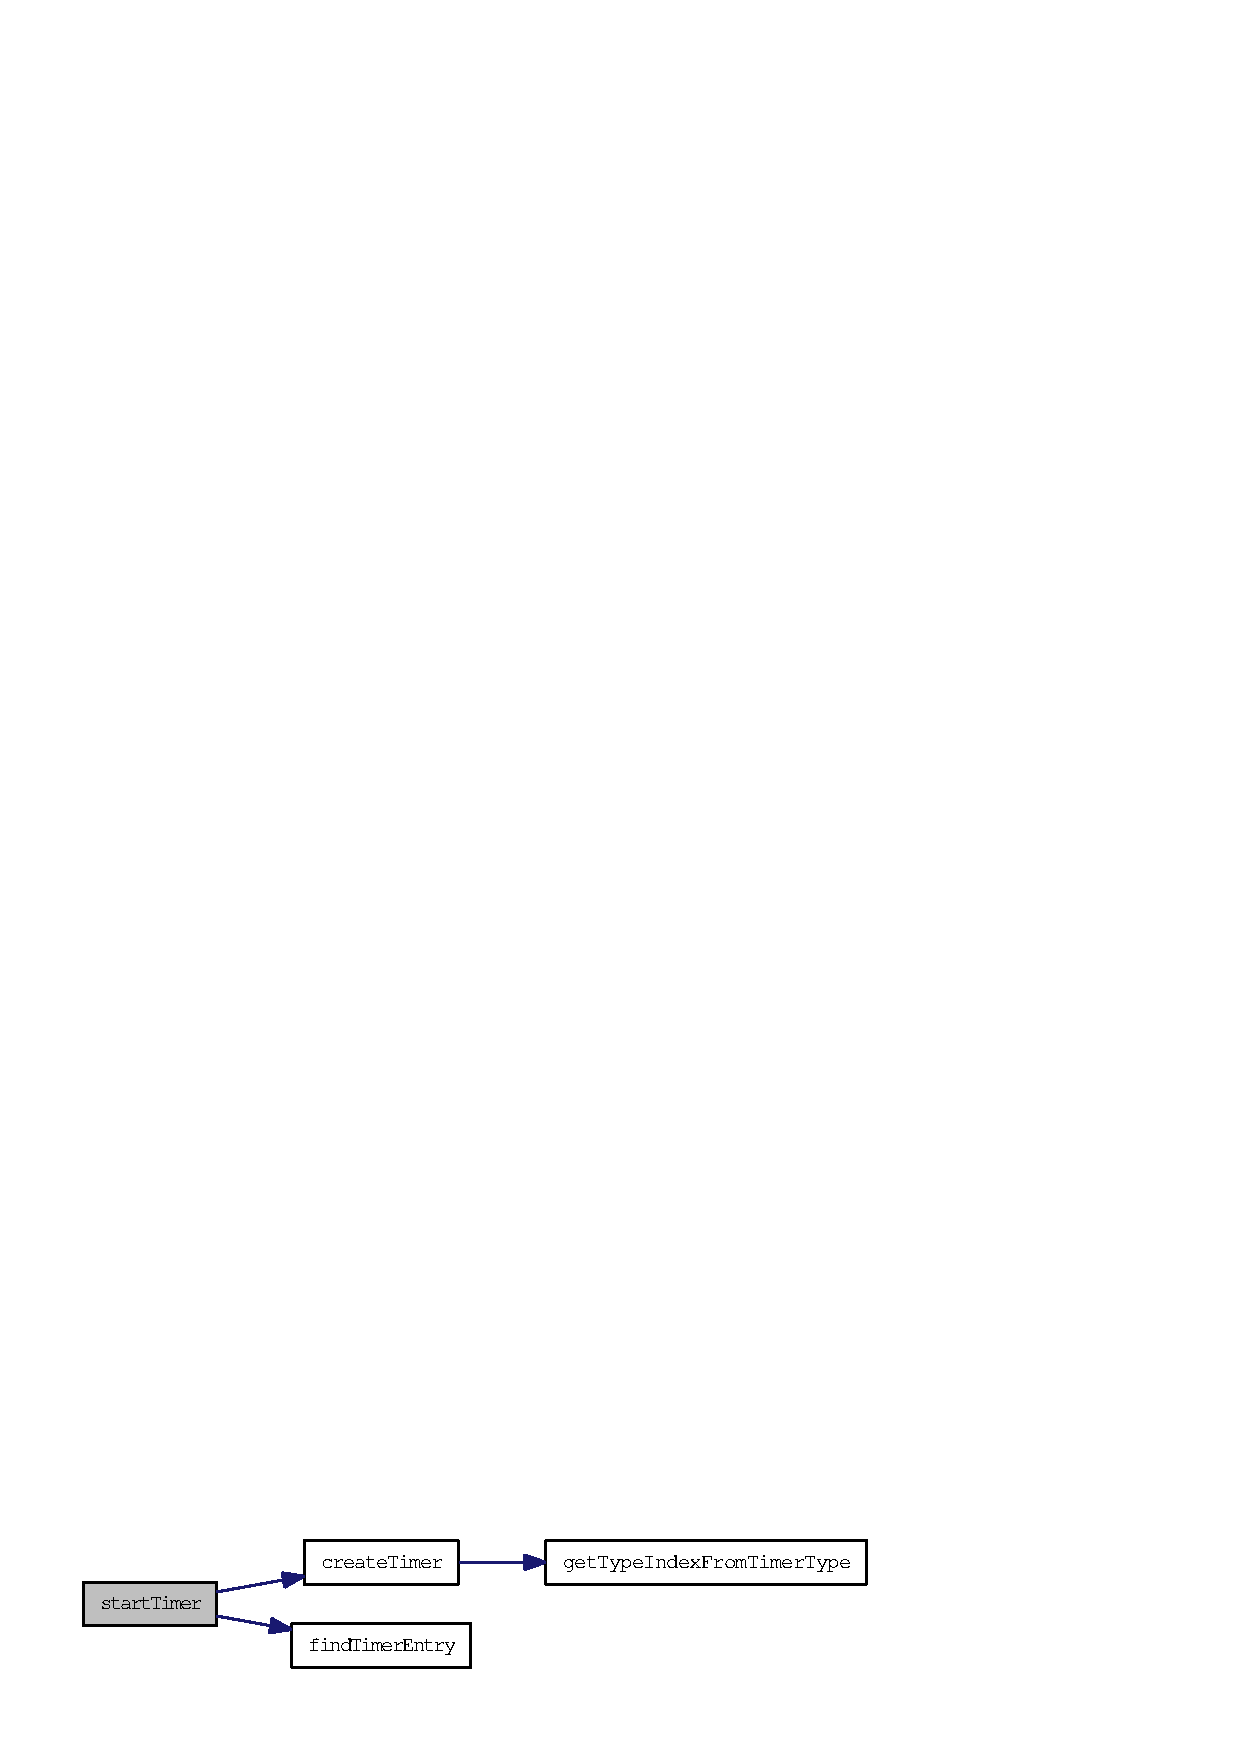
\includegraphics[width=210pt]{mrtimers_8h_ccfd598b6f1a3ca5599e8bc3588d1cf7_cgraph}
\end{center}
\end{figure}
\hypertarget{mrtimers_8h_fa991349587b8e300e5363a21dcee3b7}{
\index{mrtimers.h@{mrtimers.h}!stopTimer@{stopTimer}}
\index{stopTimer@{stopTimer}!mrtimers.h@{mrtimers.h}}
\subsubsection[stopTimer]{\setlength{\rightskip}{0pt plus 5cm}int stop\-Timer (int {\em id})}}
\label{mrtimers_8h_fa991349587b8e300e5363a21dcee3b7}




Definition at line 279 of file mrtimers.c.

References delete\-Timer().

Referenced by exec\-Batch(), exec\-Write\-Cmd(), timed\-Wait(), and wait\-Condition().

Here is the call graph for this function:\begin{figure}[H]
\begin{center}
\leavevmode
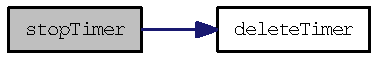
\includegraphics[width=109pt]{mrtimers_8h_fa991349587b8e300e5363a21dcee3b7_cgraph}
\end{center}
\end{figure}
